\section{Zielsetzung}
Im Versuch wird die Elktronenstrahlablenkung sowohl im elektrischen, als auch im
magnetischen Feld untersucht.

\section{Theorie}
\subsection{Erzeugung eines Elektronenstrahls}
Um einen Elektronenstrahl zu erzeugen, wird im Versuch eine sogenannte Kathodenstrahlröhre
verwendet. Diese besteht prinzipiell aus verschiedenen Komponenten, die in Abblidung \ref{abb1}
schematisch dargestellt sind. Der Elektronenstrahl wird hier über einen erhitzten Draht emittiert,
dessen Intensität vom Wehneltzylinder geregelt werden kann. Direkt dahinter befinden sich
eine Elektrode, die dazu dient, den Elektronenstrahl zu beschleunigen. Die darauf folgenden
Elektroden dienen zur Bündelung und Fokussierung des Elktronenstrahls. Zum Schluss,
vor dem Detektorschirm befinden sich zwei Plattenpaare, zwischen denen, mittels einer angelegten
Spannung, elektrische Felder entstehen, die den Elektronenstrahl zum einen horizontal (x-Richtung) und
zum anderen vertikal (y-Richuntg) ablenken können. Danach trifft der Strahl auf einen Detektorschirm, welcher
die physikalischen Eigenschaften besitzt, den auftreffenden Elektronenstrahl in Fornm eines
Leuchtflecks sichtbar zu machen.
\FloatBarrier
\begin{figure}
  \centering
  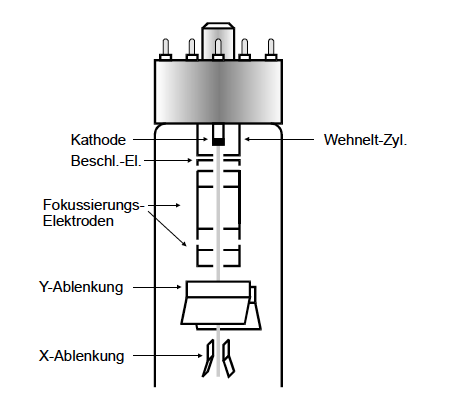
\includegraphics[scale=0.5]{kanone.PNG}
  \caption{Schematischer Aufbau der Kathodenstrahlröhre. \cite{Q1}}
  \label{abb1}
\end{figure}
\FloatBarrier
\subsection{Ablenkungen des Elektronenstrahls im elektrischen Feld}
Passiert ein Elektron ein homogenes elektrisches Feld, so wirkt auf es eine Kraft, die es ablenkt,
weshalb es zu einer Verschiebung des Auftreffpunktes auf dem Detektorschrim kommt.
In Abbildung \ref{abb2} ist der Zusammenhang zwischen der Ablenkspannung, also der Spannung,
die an den Ablenkplatten angelegt wird, und der Verschiebung D des Auftreffpunktes des
Strahls auf dem Schirm zu sehen.
Das elektrische Feld zwischen den beiden Platten kann als homogen betrachtet werden, solange
der Abstand der Platten zueinander im Verhältnis zu deren Länge klein bleibt.
Innerhalb des elektrischen Feldes wirkt dann auf ein Elktron folgende Kraft F:
\begin{align*}\label{eq1}
  F = e_0 \cdot E = e_0 \frac{U_\symup{d}}{d}
\end{align*}
\FloatBarrier
\begin{figure}
  \centering
  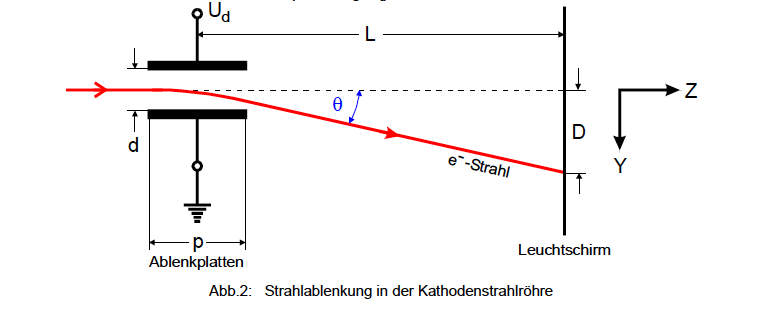
\includegraphics[scale=0.5]{abl.PNG}
  \caption{Schematischer Aufbau der Kathodenstrahlröhre. \cite{Q1}}
  \label{abb2}
\end{figure}
Der Zusammenhang zwischen Ablenkspannung und Verschiebung des Auftreffpunktes ist durch
folgende Gleichung gegeben:
\begin{align*}
  D = \frac{p}{2d} L \frac{U_\symup{d}}{U_\symup{B}}
\end{align*}
Wobei $p$ die Plattenlänge, $d$ den Plattenabstand, $L$ den Strahlweg und $U_\symup{B}$ die Beschleunigungsspannung
beschreiben.
\subsection{Erweiterung der Kathodenstrahlröhre zu einem Kathodenstrahloszillographen}
Soll auf dem Detektorschirm die Zeitabhängigkeit einer angelegten Wechselspannung dargestellt werden,
so wird dazu an die Ablenkplatte, die den Elektronenstrahl in x-richtung ablenkt (horizontal)
eine Sägezahnspannung angelegt. An die Platten, die den Strahl in y-Richtung (vertikal) ablenken,
wird die zu untersuchende Spannung angelegt.
Hierbei ist das Frequenzverhältnis der beiden angelegten Wechselspannungen zueinander von maßgeblicher
Bedeutung. Ist dieses Verhältnis korrekt aufeinander abgestimmt, so ist auf dem Detektorschirm
der zeitliche Verlauf der zu untersuchenden Wechselspannung zu sehen. Hierbei trägt die
angelegte Sägezahnspannung dazu bei, dass die Darstellung der angelgten Wechselspannung
auf dem Detektorschirm immer wieder von Neuem beginnt.
Das zu wählende Verhältnis der beiden Frequenzen ist wie folgt:
\begin{equation*}\label{eq3}
  \symup{n} \nu_\symup{s} = \symup{m} \nu_\symup{w}     ; n,m \in\mathbb{N}
\end{equation*}
\subsection{Ablenkungen des Elektronenstrahls im magnetischen Feld}
Bewegt sich ein Elektron durch ein magnetisches Feld, so wirkt auf es die Lorentzkraft:
\begin{align*}\label{eq4}
  F_\symup{L} = \symup{q} \vec \symup{v} \times \vec \symup{B}
\end{align*}
Hier ist zu erkennen, dass diese Kraft nur auftritt, wenn die Gewschwindigkeit des Elektrons
eine Komponente besitzt, die senkrecht zum B-Feld steht. Ist $\vec \symup{v}$ parallel zu
$\vec \symup{B}$, so verschwindet sie.
Der Krümmungsradius der Bahn des abgelenkten Elektrons ergibt sich, wenn die Lorentzkraft
mit der Zentrifugalkraft gleichgesetzt wird, wobei zu beachten ist, dass innerhalb des Magnetfeldes gilt, dass
$v_0 = \big| \vec v \big|$ beträgt:
\begin{align}
  r = \frac{m_0 v_0}{e_0 \symup{B}}
\end{align}
Die rechte Seite der Gleichung ist konstant, was zeigt, dass das Elektron auf einer Kreisbahn
abgelenkt wird.
\FloatBarrier
\subsection{Bestimmung der spezifischen Elektronenladung}
Mit dem Versuchsaufbau kann die spezifische Elektronenladung bestimmt werden, indem ein
Elektron mittels einer Kathodenstrahlröhre auf eine konstante Geschwindigkeit $v_0$ beschleunigt wird.
Im Feldfreienraum, flöge es nun geradlinig weiter, bis es auf den Detektroschirm trifft.
Wird mittels einer Helmholtzspule ein Magnetfeld erzeugt, wird das Elektron, wie zuvor beschrieben, abgelenkt.
Aus Abbildung \ref{abb3} geht hervor, wie der Krümungsradius mit Hilfe des Auftreffpunktes auf dem Detektorschirm
und dem Wirkungsbereich des Magnetfeldes, zu berechnen ist.
\FloatBarrier
\begin{figure}
  \centering
  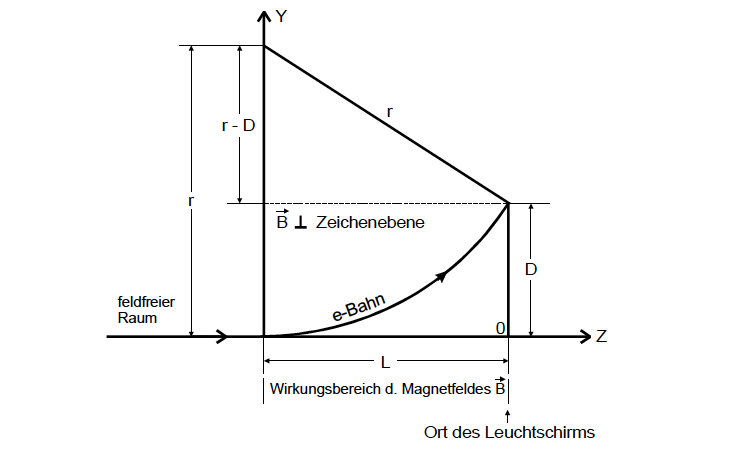
\includegraphics[scale=0.5]{abl2.PNG}
  \caption{Zusammenhang zwischen Auftreffpunkt auf dem Detektorschirm (D),
  Krümmungsradius (r) und Wirkungsbereich des Magnetfeldes (L). \cite{Q1}}
  \label{abb3}
\end{figure}
\FloatBarrier
Mit Hilfe der Formel für die Geschwindigkeit des Elektrons $v_0$, die mittels der Beschleunigungsspannung $U_\symup{B}$
berechnet wird:
\FloatBarrier
\begin{align*}\label{eq6}
  v_0 = \sqrt{2 U_\symup{B} e_0/m_0}
\end{align*}
\FloatBarrier
und Gleichung \ref{eq5}, kann dann die spezifische Elektronenladung bestimmt werden:
\FloatBarrier
\begin{align*}
  \frac{e_0}{m_0} = \frac{8 U_\symup{B} D^2}{\left(\symup{L}^2 + \symup{D}^2\right)\symup{B}^2}.
\end{align*}

\section{Durchführung}
Im ersten Teil des Versuchs wird die Proportionalität zwischen der Ablenkspannung und der
Verschiebung des Auftreffpunktes auf dem Detektorschirm untersucht. Hierbei werden
fünf verschiedene Beschleunigungsspannungen verwendet. Bei denen jeweils die Ablenkspannung
so geregelt wird, dass der Leuchtfleck auf neun verschiedene äquidistante Linien
auf dem Detektorschirm zu sehen ist. Die zugehörigen Spannungen werden notiert.
Die zur Messung gehörige Schaltung ist in Abbildung \ref{abb4} zu sehen.
\begin{figure}
  \centering
  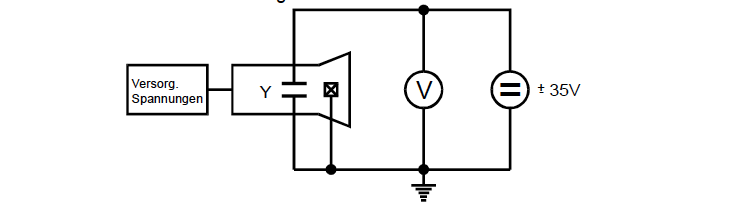
\includegraphics[scale=0.5]{abl3.PNG}
  \caption{Schaltung für die Untersuchung der Proportionalität zwischen Ablenkspannung
  und Verschiebung des Auftreffpunktes. \cite{Q1}}
  \label{abb4}
\end{figure}
\FloatBarrier

\noindent Im zweiten Teil wird ein einfacher Kathodenstrahloszillograph gebaut. Die zugehörige Schaltung
ist in Abbildung \ref{abb5} zu sehen. Hierbei wird die Sägezahnfrequenz so geregelt, dass auf dem Oszillographen
stehende Bilder der Sinusspannung zu sehen sind. Es werden vier verschiedene Vielfache $n$ der
Sägezahnspannung untersucht: $ n = \frac{1}{2}, 1, 2, 3$. Die exakte Frequenz wird am
Frequenzzähler abgelesen. Bei konstanter Beschleunigungsspannung wird des Weiteren die Amplitude
der stehenden Sinuswelle bei allen vier Frequenzvielfachen abgelesen.
\FloatBarrier
\begin{figure}
  \centering
  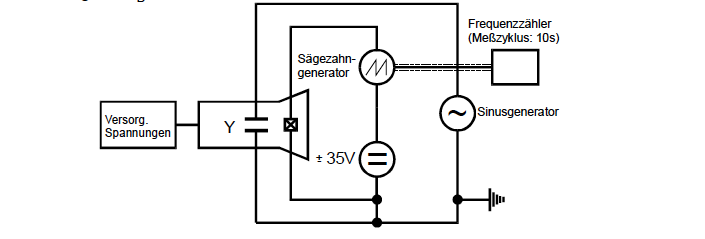
\includegraphics[scale=0.5]{abl4.PNG}
  \caption{Schaltung zum Bau eines einfachen Kathodenstrahloszillographen. \cite{Q1}}
  \label{abb5}
\end{figure}
\FloatBarrier
\noindent Im dritten Teil des Doppelversuchs wird nun die spezifische Elektronenladung
mittels der Ablenkung des Elektronenstrahls im Magnetfeld ermittelt.
Hierzu wird durch eine Helmholtzspule ein homogenes Magnetfeld erzeugt, das senkrecht zur Kathodenstrahlröhre
ausgerichtet wird.
Das entsehende Magnetfeld ist in der Versuchsanleitung \ref{Q1} angegeben:
\begin{align*}
  B = \mu_0 \frac{8}{\sqrt{125}} \frac{\symup{N} \cdot I }{R}.
\end{align*}
Des Weiteren ist zu beachten, dass die Achse der Kathodenstrahlröhre in Richtung der Horizontalkomponente
des Erdmagnetfeldes ausgerichtet wird. Um die Feldrichtung zu ermitten, steht ein spezieller
Kompass (Deklinatorium/Inklinatorium) bereit.
Anschließend wird bei fünf verschiedenen, konstanten Beschleunigungsspannungen die Strahlverschiebung D
in Abhängigkeit vom, durch den Strom $I$ erzeugten, magnetischen Feld untersucht. Hierzu wird der Strom $I$
neun mal so eingestellt, dass der Auftreffpunkt der Elektonen auf dem Detektorschirm auf neun verschiedenen
äquidistanten Linien zu sehen ist. Der zugehörige Strom zum Auftreffpunkt D werden notiert.

\noindent Im letzten Teil des Versuchs wird die Intensität des Magnetfeldes am Versuchsort ermittelt.
Hierzu wird zunächst der Inklinationswinkel $\varphi$ ermittelt, welcher der Winkel zwischen Horizontalebene
und der Richtung des Erdfeldes ist. Hierzu wird das Inklinatorium um seine vertikale Achso so gedreht, dass
dessen Nadel in Nord-/Südrichtung zeigt. Anschließend wird der Teilkreis des Inklinatoriums um $\SI{90}{\degree}$
gedreht. Nun zeigt die Nadel in Richtung des Erdfeldes. Diese Messung wird dreimal durchgeführt, um eventuelle
Messfehler zu minimieren.
Anschließend wird bei einer konstanten Beschleunigungsspannung und ausgeschaltetem Magnetfeld
die Kathodenstrahlröhre so ausgerichtet, dass sie in die, zuvor mit Hilfe des Inklinatoriums ermittelte,
Nord-/Südrichtung zeigt. Die Lage des Leuchtflecks auf dem Detektorschirm wird exakt notiert und sich gemerkt.
Im Anschluss wird die Versuchsanordnung in Ost-/Westrichtung ausgerichtet, sodass nun das Erdfeld eine
Ablenkung des Elektronenstrahls verursacht. Nun wird die Helmholtzspule angeschaltet und
der Strom $I$ so reguliert, dass das so erzeugte Magnetfeld dem der Erde entgegenwirkt und sich
der Leuchtfleck auf dem Detektorschirm wieder an der gleichen Stelle befindet, wie zu Anfang des Versuchteils.
Der benötigte Strom $I$ wird notiert.
